\documentclass[tikz, border=10pt]{standalone}
\usepackage{amsmath}
\usepackage{tikz}
\usetikzlibrary{decorations.pathmorphing, arrows.meta, calc, backgrounds}

\definecolor{navybg}{RGB}{13,27,42}
\definecolor{source1col}{RGB}{0,220,255}
\definecolor{source2col}{RGB}{255,165,0}
\definecolor{labelcol}{RGB}{220,220,220}
\definecolor{plotbg}{RGB}{25,40,60}
\definecolor{axiscol}{RGB}{180,180,180}
\definecolor{thirdcol}{RGB}{100,255,150}

\begin{document}
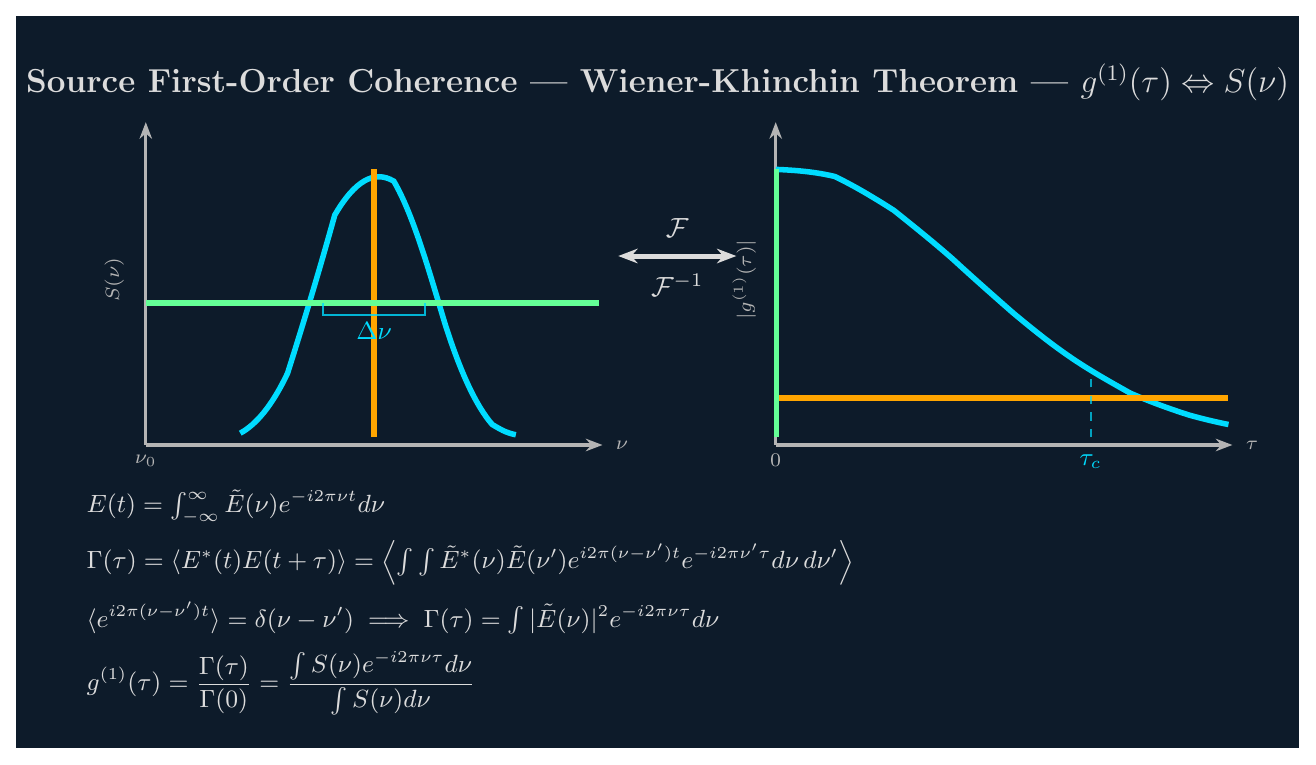
\begin{tikzpicture}[
    background rectangle/.style={fill=navybg},
    show background rectangle,
    arr/.style={-{Stealth[length=6pt]}, line width=1.2pt},
    arrthin/.style={-{Stealth[length=4pt]}, line width=0.8pt},
]

\path[use as bounding box] (0,0) rectangle (16,9);

% ════════════════════════════════════════════════════════
% 0. TITLE
% ════════════════════════════════════════════════════════
\node[text=labelcol, font=\large\bfseries] at (8.0, 8.3)
    {Source First-Order Coherence \textemdash\ Wiener-Khinchin Theorem \textemdash\
     $g^{(1)}(\tau) \Leftrightarrow S(\nu)$};

% ════════════════════════════════════════════════════════
% 1. LEFT PANEL: |g^(1)(τ)| COHERENCE FUNCTION
% ════════════════════════════════════════════════════════
\coordinate (COHERENCE) at (9.5, 3.8);

% Axes
\draw[arr, axiscol] ($(COHERENCE)+(0,-0.1)$) -- ($(COHERENCE)+(5.8,-0.1)$);
\draw[arr, axiscol] ($(COHERENCE)+(0,-0.1)$) -- ($(COHERENCE)+(0, 4.0)$);
\node[text=axiscol, font=\scriptsize] at ($(COHERENCE)+(6.05,-0.1)$) {$\tau$};
\node[text=axiscol, font=\scriptsize, rotate=90] at ($(COHERENCE)+(-0.4, 2.0)$) {$|g^{(1)}(\tau)|$};
\node[text=axiscol, font=\scriptsize] at ($(COHERENCE)+(0.0,-0.3)$) {$0$};

% Cyan — narrow spectrum, long coherence time τ_c1 ≈ 4 (plot units)
% Gaussian envelope: 3.4 * exp(-(x/4)^2)
% x=0:3.40, x=0.5:3.37, x=1:3.19, x=1.5:2.88, x=2:2.48, x=2.5:2.03,
% x=3:1.59, x=3.5:1.18, x=4:0.84, x=4.5:0.56, x=5:0.36, x=5.5:0.21
\draw[source1col, line width=2pt]
    ($(COHERENCE)+(0.0,  3.40)$)
    .. controls ($(COHERENCE)+(0.25, 3.39)$) and ($(COHERENCE)+(0.5,  3.37)$) ..
    ($(COHERENCE)+(0.75, 3.31)$)
    .. controls ($(COHERENCE)+(1.0,  3.19)$) and ($(COHERENCE)+(1.25, 3.04)$) ..
    ($(COHERENCE)+(1.5,  2.88)$)
    .. controls ($(COHERENCE)+(1.75, 2.68)$) and ($(COHERENCE)+(2.0,  2.48)$) ..
    ($(COHERENCE)+(2.25, 2.26)$)
    .. controls ($(COHERENCE)+(2.5,  2.03)$) and ($(COHERENCE)+(2.75, 1.81)$) ..
    ($(COHERENCE)+(3.0,  1.59)$)
    .. controls ($(COHERENCE)+(3.25, 1.38)$) and ($(COHERENCE)+(3.5,  1.18)$) ..
    ($(COHERENCE)+(3.75, 1.01)$)
    .. controls ($(COHERENCE)+(4.0,  0.84)$) and ($(COHERENCE)+(4.25, 0.70)$) ..
    ($(COHERENCE)+(4.5,  0.56)$)
    .. controls ($(COHERENCE)+(4.75, 0.45)$) and ($(COHERENCE)+(5.0,  0.36)$) ..
    ($(COHERENCE)+(5.25, 0.28)$)
    .. controls ($(COHERENCE)+(5.5,  0.21)$) and ($(COHERENCE)+(5.7,  0.17)$) ..
    ($(COHERENCE)+(5.75, 0.16)$);

% Orange — delta function spectrum → constant |g^(1)| = 1 (perfect coherence)
\draw[source2col, line width=2pt]
    ($(COHERENCE)+(0.0, 0.5)$) -- ($(COHERENCE)+(5.75, 0.5)$);

% Green — constant (white) spectrum → delta function coherence at τ=0
\draw[thirdcol, line width=2pt]
    ($(COHERENCE)+(0.01, 3.40)$) -- ($(COHERENCE)+(0.01, 0.0)$);

% τ_c annotation for cyan
\draw[source1col, line width=0.8pt, dashed, opacity=0.7]
    ($(COHERENCE)+(4.0, 0.0)$) -- ($(COHERENCE)+(4.0, 0.84)$);
\node[text=source1col, font=\small, below=3pt] at ($(COHERENCE)+(4.0, 0.0)$) {$\tau_c$};

% ════════════════════════════════════════════════════════
% 2. FOURIER TRANSFORM ARROW (CENTER)
% ════════════════════════════════════════════════════════
\draw[{Stealth[length=7pt]}-{Stealth[length=7pt]}, line width=1.8pt, labelcol]
    (7.5, 6.1) -- (9.0, 6.1);
\node[text=labelcol, font=\normalsize, above=3pt] at (8.25, 6.1) {$\mathcal{F}$};
\node[text=labelcol, font=\normalsize, below=3pt] at (8.25, 6.1) {$\mathcal{F}^{-1}$};

% ════════════════════════════════════════════════════════
% 3. RIGHT PANEL: S(ν) POWER SPECTRUM
% ════════════════════════════════════════════════════════
\coordinate (SPECTRUM) at (1.5, 3.8);

% Axes
\draw[arr, axiscol] ($(SPECTRUM)+(0,-0.1)$) -- ($(SPECTRUM)+(5.8,-0.1)$);
\draw[arr, axiscol] ($(SPECTRUM)+(0,-0.1)$) -- ($(SPECTRUM)+(0, 4.0)$);
\node[text=axiscol, font=\scriptsize] at ($(SPECTRUM)+(6.05,-0.1)$) {$\nu$};
\node[text=axiscol, font=\scriptsize, rotate=90] at ($(SPECTRUM)+(-0.4, 2.0)$) {$S(\nu)$};
\node[text=axiscol, font=\scriptsize] at ($(SPECTRUM)+(0.0,-0.3)$) {$\nu_0$};

% Both peaks centered at x=2.9 (ν₀)
% Cyan — narrow Gaussian, σ=0.55, peak=3.4
% x=1.2:0.05, x=1.6:0.39, x=2.0:1.44, x=2.4:2.82, x=2.9:3.40,
% x=3.4:2.82, x=3.8:1.44, x=4.2:0.39, x=4.6:0.05
\draw[source1col, line width=2pt]
    ($(SPECTRUM)+(1.2,  0.05)$)
    .. controls ($(SPECTRUM)+(1.4,  0.16)$) and ($(SPECTRUM)+(1.6,  0.39)$) ..
    ($(SPECTRUM)+(1.8,  0.81)$)
    .. controls ($(SPECTRUM)+(2.0,  1.44)$) and ($(SPECTRUM)+(2.2,  2.10)$) ..
    ($(SPECTRUM)+(2.4,  2.82)$)
    .. controls ($(SPECTRUM)+(2.65, 3.25)$) and ($(SPECTRUM)+(2.9,  3.40)$) ..
    ($(SPECTRUM)+(3.15, 3.25)$)
    .. controls ($(SPECTRUM)+(3.4,  2.82)$) and ($(SPECTRUM)+(3.6,  2.10)$) ..
    ($(SPECTRUM)+(3.8,  1.44)$)
    .. controls ($(SPECTRUM)+(4.0,  0.81)$) and ($(SPECTRUM)+(4.2,  0.39)$) ..
    ($(SPECTRUM)+(4.4,  0.16)$)
    .. controls ($(SPECTRUM)+(4.55, 0.07)$) and ($(SPECTRUM)+(4.6,  0.05)$) ..
    ($(SPECTRUM)+(4.7,  0.03)$);

% Orange — delta function spectrum: spike at ν₀
\draw[source2col, line width=2pt]
    ($(SPECTRUM)+(2.9, 0.0)$) -- ($(SPECTRUM)+(2.9, 3.40)$);

% Green — constant (white) spectrum: flat line
\draw[thirdcol, line width=2pt]
    ($(SPECTRUM)+(0.0, 1.70)$) -- ($(SPECTRUM)+(5.75, 1.70)$);

% Bandwidth annotation for cyan only
\draw[source1col, line width=0.8pt, opacity=0.8]
    ($(SPECTRUM)+(2.25, 1.70)$) -- ($(SPECTRUM)+(2.25, 1.55)$)
    -- ($(SPECTRUM)+(3.55, 1.55)$) -- ($(SPECTRUM)+(3.55, 1.70)$);
\node[text=source1col, font=\small] at ($(SPECTRUM)+(2.9, 1.35)$) {$\Delta\nu$};

% ════════════════════════════════════════════════════════
% 4. CAPTION
% ════════════════════════════════════════════════════════
\node[text=labelcol, font=\small, align=left, text width=14.5cm] at (8.0, 1.7)
    {$E(t) = \int_{-\infty}^{\infty} \tilde{E}(\nu) e^{-i2\pi\nu t} d\nu$ \\[5pt]
     $\Gamma(\tau) = \langle E^*(t) E(t+\tau) \rangle = \left\langle \int \int \tilde{E}^*(\nu) \tilde{E}(\nu') e^{i2\pi(\nu-\nu') t} e^{-i2\pi\nu'\tau} d\nu \, d\nu' \right\rangle$ \\[5pt]
     $\langle e^{i2\pi(\nu-\nu')t}\rangle = \delta(\nu - \nu') \implies \Gamma(\tau) = \int |\tilde{E}(\nu)|^2 e^{-i2\pi\nu\tau} d\nu$ \\[5pt]
     $g^{(1)}(\tau) = \dfrac{\Gamma(\tau)}{\Gamma(0)} = \dfrac{\int S(\nu) e^{-i2\pi\nu\tau} d\nu}{\int S(\nu) d\nu}$};

\end{tikzpicture}
\end{document}
